\documentclass{article}
\usepackage{graphicx}
\usepackage{color}

\usepackage{alltt}
\usepackage{amssymb,amsmath,natbib,graphicx,enumerate,subcaption,tikz,url,booktabs}
\usepackage[bmargin=0.75in, tmargin =0.75in,lmargin = 0.5in,rmargin = 0.5in]{geometry}

\usepackage{dsfont}
\usepackage[ruled]{algorithm2e}
\usepackage{algpseudocode}
\renewcommand{\algorithmcfname}{Procedure}
\usepackage{bbold}


\newcommand{\ith}{i^\textrm{th}}
\newcommand{\CVE}{\textrm{CVE}}
\newcommand{\MSE}{\textrm{MSE}}
\newcommand{\logit}{\mbox{logit}}
\newcommand{\E}{\mathbb{E}}
\newcommand{\Prob}{\mathbb{P}}
\newcommand{\ones}{\mathbbm{1}}
\newcommand{\indic}[1]{\boldsymbol{1}_{\{ #1 \}}}
\newcommand{\mvec}{\mbox{vec}}
\newcommand{\cov}{\mbox{Cov}}
\newcommand{\eqdist}{\overset{{\cal D}}{=}}
\newcommand{\const}{\mbox{const}}
\newcommand{\iid}{\overset{iid}{\sim}}
\newcommand{\diag}{\mbox{{\bf diag}}}
\newcommand{\Diag}{\mbox{Diag}}
\providecommand{\Tr}{^{\scriptscriptstyle\top}}

\newcommand{\lam}{\lambda}
\newcommand{\bmu}{\boldsymbol\mu}
\newcommand{\balpha}{\boldsymbol\alpha}
\newcommand{\br}{\boldsymbol{r}}
\newcommand{\bs}{\boldsymbol{s}}
\newcommand{\by}{\boldsymbol{y}}
\newcommand{\bbeta}{\boldsymbol{\beta}}
\newcommand{\btheta}{\boldsymbol{\theta}}
\newcommand{\btau}{\boldsymbol{\tau}}
\newcommand{\bx}{\boldsymbol{x}}
\newcommand{\beps}{\boldsymbol\epsilon}

\newcommand{\cX}{{\cal X}}
\newcommand{\cA}{{\cal A}}
\newcommand{\cAmin}{{\cal A}^{\mathsmaller{-}}}

\newcommand{\vm}[1]{\mbox{vec}^\mathsmaller{-}\hspace{-0.25pc}\left(#1\right)}
\newcommand{\Imin}{I^\mathsmaller{-}}
\newcommand{\Itri}{{I^\mathsmaller{\triangle}}}

\newcommand{\deriv}[1]{\noindent {\it Derivation:} #1 $\hfill\square$}
\newcommand{\pbe}[1]{{\cal P}_{\epsilon,#1}}
\newcommand{\be}{{\cal B}_{\epsilon}}

\newcommand{\adjSet}{\{A_{k_\ell}\}_{\ell=1}^K}
\newcommand{\abSet}{\{\alpha_{k_\ell},\bbeta_{k_\ell}\}_{\ell=1}^K}
\newcommand{\bZ}{{\bf Z}}

\providecommand{\note}[1]{\textcolor{red}{#1}}
\providecommand{\bnote}[1]{\textcolor{blue}{#1}}

\title{Supporting Information\\
\textit{Cross Validation Approaches for Penalized Cox Regression}}

\author{Biyue Dai\\Department of Biostatistics\\University of Iowa
  \and
  Patrick Breheny\\Department of Biostatistics\\University of Iowa}
\date{\today}

\IfFileExists{upquote.sty}{\usepackage{upquote}}{}

\begin{document}
\maketitle

\section{Baseline Estimation for Cross-Validated Deviance Residuals}

As described in the manuscript, the Martingale residuals $\{m_i\}_{i=1}^n$ and deviance residuals $\{d_i\}_{i=1}^n$ for the Cox model are given by
\begin{align*}
  m_{i} &= \delta_{i} - H_{0}(t_{i})\exp(X_i\Tr\beta) \\
  d_{i} &= \text{sign}(m_{i})\sqrt{-2(m_i + \delta_{i}\log(\delta_{i} - m_i))},
\end{align*}
where $H_0$ is the cumulative baseline hazard.  Our cross-validated versions of these residuals use
\begin{align*}
  m_{i}^{cv} &= \delta_{i} - \hat{H}_{0}(t_{i})\exp(X_i\Tr\hat\beta^{-k}) \\
  d_{i}^{cv} &= \text{sign}(m_{i}^{cv})\sqrt{-2(m_i^{cv} + \delta_{i}\log(\delta_{i} - m_i^{cv}))},
\end{align*}
for $i$ in the test set $D_k$, with $\hat{\beta}^{-k}$ obtained from the training set $T_k$.  The sum of squared cross-validated deviance residuals, $\sum_{i}(d_{i}^{cv})^2$, are then used as the cross validated error, analogously to using the residual sum of squares in linear regression.  In the manuscript, this method is referred to as the \emph{cross-validated deviance residuals} approach.

%Deviance residuals are typically calculated based on a baseline hazard estimate that has been adjusted for the covariates in the model. In the context of cross-validation, however, this approach is problematic. Deviance residuals measure the difference between the fitted model and a saturated model; in Cox regression, this saturated model depends on the baseline hazard. Thus, a covariate-adjusted baseline hazard would mean that each fold is compared to a different saturated model. For this reason, it is important that the baseline hazard remains constant across folds when calculating cross-validated deviance residuals; this intuition is borne out by simulations involving various other possible ways of constructing cross-validated deviance residuals.  

\subsection{Baseline Estimations}

	\subsubsection{Nelson-Aalen Estimator}
	 The simplest approach to estimating the cumulative baseline hazard, $H_0$, is the Nelson-Aalen Estimator \citep{nelson1969, aalen1978}:
\begin{equation}
  \hat{H}_{0}(t) = \sum_{t_j \leq t}\frac{\text{number of failures at time } t_j}{\text{number at risk right before time }t_j}.
\end{equation}
Under the assumption that there is no ties among failure times, the numerator in the summation is either 0 or 1. The Nelson-Aalen Estimator depends only on the failure times and does not involve any information from the covariates. Procedure~\ref{alg:na} provides an explicit description of this algorithm.

\begin{algorithm}
\SetAlgoLined
Use all observations' time and status to compute $\hat{H}_{0}(t) = \sum_{t_j \leq t}\frac{\text{number of failures at time } t_j}{\text{number at risk right before time }t_j}$\;
\For{each regularization parameter $\lambda$}{
 \For{each fold $k = 1,2,...,K$}{
  Use the training set $T_k$ to obtain $\hat{\beta}^{-k}$\;
  	\For{each obervation $i$ in the $k$th fold}{
  	Compute the Cross-validated Martingale Residual: $\hat{M}^{cv}_{i}  = \delta_{i} - \hat{H}_{0}(t_{i})\exp(X_i\Tr\hat\beta^{-k})$\;
  	Compute the Deviance Residual: $ d_{i} = \text{sgn}(\hat{M}^{cv}_{i})\sqrt{-2(\hat{M}^{cv}_{i} + \delta_{i}\log(\delta_{i} - \hat{M}^{cv}_{i}))}$\;
  	}
 }
 Compute the sum of squares: $\sum_{i}\hat{d}_{i}^2$
 }
 \caption{\label{alg:na} Compute cross-validated deviance residuals based on the Nelson-Aalen estimator}
\end{algorithm}
	
\subsubsection{Breslow's Approach}	
	
In the original proposal of the Martingale Residuals \citep{Therneau1990}, Breslow's estimator \citep{Breslow1974} was the prefered approach for estimating the cumulative baseline hazard. Under the assumption that there is no ties among the failure times, the Breslow's estimator is defined as:
\begin{equation} 
\hat{H}_0(t) = \sum_{t_{i} \leq t}\frac{\delta(t_i)}{\sum_{ j \in R(t_{i})}\exp (\hat{\eta}_{j})}.
\end{equation}
Covariates of the fitted model are incorporated in the denominator of the summation.
Procedure~\ref{alg:brkp} includes an explicit description of this algorithm.
\begin{algorithm}
\SetAlgoLined
\For{each regularization parameter $\lambda$}{
 Fit the model using all observations' time and status \;
 Obtain linear predictor $\hat{\eta}$ from the fitted model\;
 \uIf{Use the Breslow's estimator}{
 $\hat{H}_0(t) = \sum_{t_{i} \leq t}\frac{\delta(t_i)}{\sum_{ j \in R(t_{i})}\exp (\hat{\eta}_{j})}$;
 }\ElseIf{Use the Kalbfleisch and Prentice estimator}{
  $\hat{H}_0(t) = \sum_{t_{i} \leq t} \left\{1 -  \left(1 - \frac{\exp (\hat{\eta}_{i})}{\sum_{ j \in R(t_{i})}\exp (\hat{\eta}_{j})} \right) ^{\exp(-\hat{\eta}_{i})}\right\}$\;
 }
 \For{each fold $k = 1,2,...,K$}{
  Use the training set $T_k$ to obtain $\hat{\beta}^{-k}$\;
  	\For{each obervation $i$ in the $k$th fold}{
  	Compute the Cross-validated Martingale Residual: $\hat{M}^{cv}_{i}  = \delta_{i} - \hat{H}_{0}(t_{i})\exp(X_i\Tr\hat\beta^{-k})$\;
  	Compute the Deviance Residual: $ d_{i} = \text{sgn}(\hat{M}^{cv}_{i})\sqrt{-2(\hat{M}^{cv}_{i} + \delta_{i}\log(\delta_{i} - \hat{M}^{cv}_{i}))}$\;
  	}
 }
 Compute the sum of squares: $\sum_{i}\hat{d}_{i}^2$
 }
 \caption{\label{alg:brkp} Compute cross-validated deviance residuals based on the Breslow estimator and the Kalbfleisch and Prentice estimator}
\end{algorithm}

\subsubsection{Kalbfleisch and Prentice's Approach}					

\cite{Kalbfleisch2011} proposed a cumulative hazard estimator that incorporates covariates. Assuming only a single failure occurs at $t_i$, based on the fitted values of $\hat{\bbeta}$, we can first compute linear predictors $\hat{\eta}_i$ at each observed failure time. Based on $\hat{\eta}_i$, we can compute a discrete hazard component at each observed failure time):
\begin{equation}
1 - \hat{\alpha}_{i} = 1 - \left( 1 - \frac{\exp (\hat{\eta}_{i})}{\sum_{ j \in R(t_{i})}\exp (\hat{\eta}_{j})} \right)^{\exp(-\hat{\eta}_{i})},
\end{equation}
and aggregate them together into the cumulative hazard function:
\begin{equation} 
\hat{H}_0(t) = \sum_{t_{i} \leq t}(1 - \hat{\alpha}_i),
\end{equation}
Procedure~\ref{alg:brkp} includes an explicit description of this algorithm.

\subsection{Simulation Comparison}
The following simulation illustrates how the performance of cross-validated deviance residuals would vary based on different baseline estimation. We generated data using the same mechanism as we described in Section 3.1 in the paper. In each simulated data set, there were $n = 150$ observations, $p = 1000$ number of feature and 10 non-zero features with signal strength $s$. Censoring proportion is fixed at $10\%$. For each scenario, we varied $s$ from 0.4 to 0.9 and 200 replications were used. We compared the cross-validated deviance residuals constructed by Nelson-Aalen estimator and the cross-validated deviance residuals constructed by Kalbfleisch and Prentice's estimator. We also included cross-validated linear predictor approach (introduced in Section 2.3 in the paper) for comparison. The results of the simulation is listed in the following table:

\begin{table}[h]
\centering
\begin{tabular}{lrrrrrr}
\toprule
  & 0.4 & 0.5 & 0.6 & 0.7 & 0.8 & 0.9\\
\midrule
\vspace{1mm}
 & \multicolumn{5}{c}{$\lambda$} & \\ 
\vspace{1mm}
Nelson Aalen & 0.152 & 0.134 & 0.127 & 0.121 & 0.121 & 0.121\\
Breslow & 0.258 & 0.247 & 0.228 & 0.199 & 0.178 & 0.165\\
Kalbfleisch and Prentice & 0.249 & 0.234 & 0.210 & 0.180 & 0.155 & 0.144\\
%CVLP & 0.1441 & 0.1214 & 0.1078 & 0.0981 & 0.0914 & 0.0849\\
%Oracle &  0.1090 & 0.0941 & 0.0762 & 0.0615 & 0.0567 & 0.0516\\
\vspace{0.5mm}\\
 & \multicolumn{5}{c}{$\log($MSE Ratio$)$} & \\ 
\vspace{1mm}
Nelson Aalen & 2.431 & 2.624 & 2.806 & 2.983 & 3.186 & 3.346 \\
Breslow & 2.729 & 3.074 & 3.301 & 3.449 & 3.562 & 3.632 \\
Kalbfleisch and Prentice & 2.712 & 3.034 & 3.232 & 3.355 & 3.427 & 3.508 \\
%CVLP &2.3684 & 2.4089 & 2.6595 & 2.7173 & 2.7761 & 2.8264\\
\bottomrule
\end{tabular}
\end{table}

Top half of the table listed different $\lambda$ values selected by the method. With the Kalbfleisch and Prentice baseline, the cross-validated deviance residual always selected larger $\lambda$ values and very conservative models. With the covariate-adjusted baseline, the deviance residuals seem to have stronger preference for models closer to the null model. This phenomenon is also observed by the original authors of the deviance residuals in classical Cox regression applications. As they attempted to use the covariate-adjusted deviance residuals and Martingale residuals to evaluate model fit, they observed that "the no-covariate model has the smallest sum of squared and the best model, the one with all five predictors, has the largest" \citep{Therneau2000modeling}.

The bottom half of the table listed $\log($MSE Ratio$)$ of the models selected by cross-validation approaches compared to the oracle model. The definition of $\log($MSE Ratio$)$ is described in more details in Section 3.1 in the paper. Throughout different signal strength, CVDR with Kalbfleisch and Prentice baseline had the largest $\log($MSE Ratio$)$, indicating worst model estimation among all methods. With Nelson-Aalen estimator, the CVDR approach had better performance and performed closer to CVLP at weaker signals. As the signal strength increases, the performance of CVDR with Nelson-Aalen estimator also declined.

Overall, our simulation results support the use of Nelson-Aalen estimator in estimating the baseline hazard for the cross-validated deviance residual approach.

\section{Simulation with Correlated Features}

Simulations in this section are conducted to examine how correlations among features can impact the performance of the cross-validation approaches.

The data generating mechanism is similar to simulations presented in Figure 2 in the manuscript, except that each non-zero feature is correlated with 10 null features. We considered two types of correlation structures: exchangeable and autoregressive. We simulated data with a spectrum of correlation, from 0 to 0.8. Results of the simulation is presented in Figure~\ref{Fig:ex} for exchangeable correlation structure and Figure~\ref{Fig:auto} for autoregressive correlation structure.

\begin{figure}[ht]
  \centering
  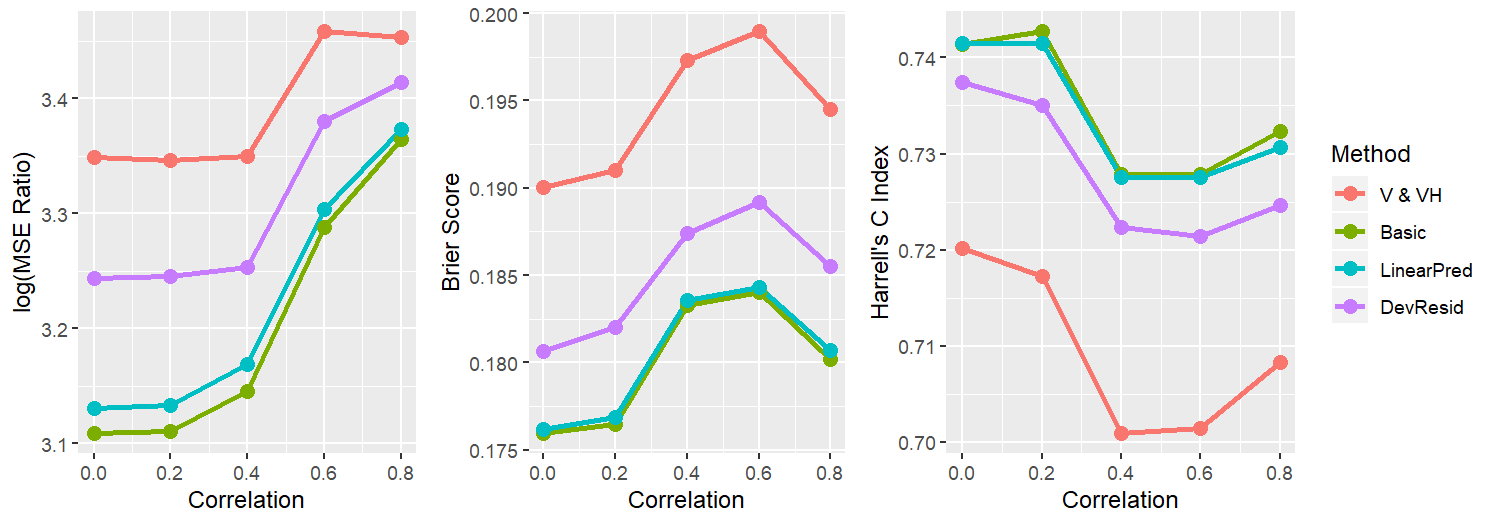
\includegraphics[width=\textwidth]{manuscript_figure/figure_2_ex.png}
  \caption{\label{Fig:ex} The horizontal axis in all three plots is the correlation among the features. The value of $s$ is varied from 0.4 to 0.9.  $\log(\text{MSE ratio})$, relative to the oracle modle is plotted in the left panel. Out-of-sample Brier scores are plotted in the middle. Out-of-sample C index is plotted in the right panel. For each simulated data set, n = 120, p = 1000. Expected censoring percentage is 10$\%$.}
\end{figure}	

\begin{figure}[ht]
  \centering
  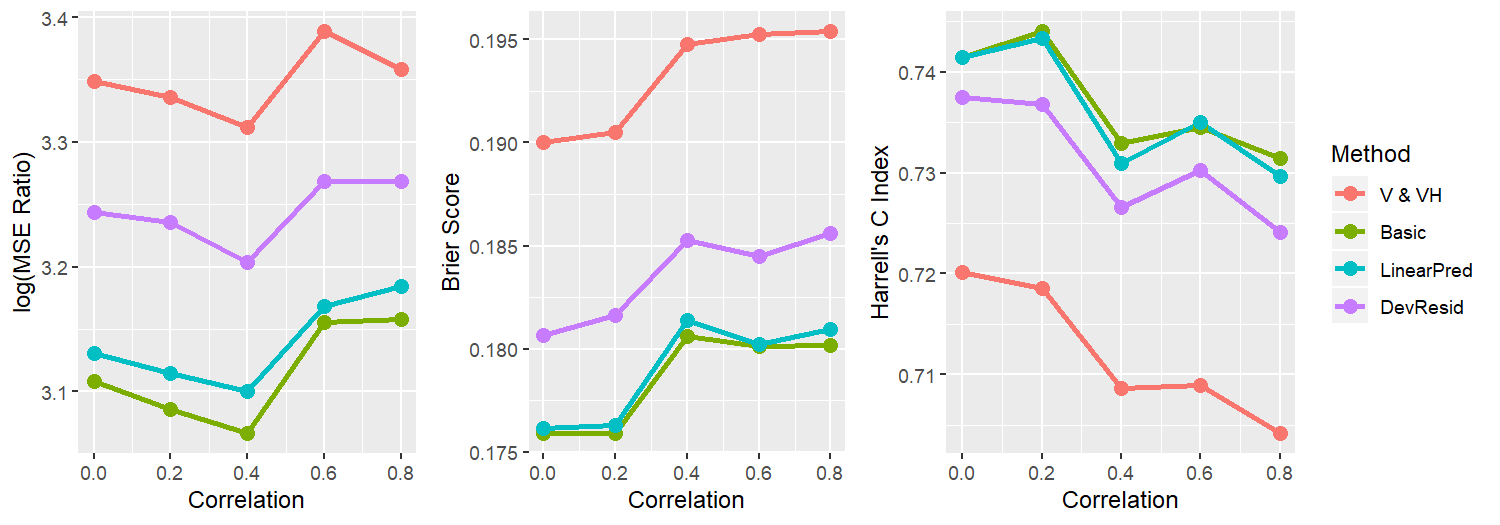
\includegraphics[width=\textwidth]{manuscript_figure/figure_2_auto.png}
  \caption{\label{Fig:auto} The horizontal axis in all three plots is the correlation among the features. The value of $s$ is varied from 0.4 to 0.9.  $\log(\text{MSE ratio})$, relative to the oracle modle is plotted in the left panel. Out-of-sample Brier scores are plotted in the middle. Out-of-sample C index is plotted in the right panel. For each simulated data set, n = 120, p = 1000. Expected censoring percentage is 10$\%$.}
\end{figure}	

As is shown in the figures, across different correlation structure and strength of the correlation, the basic approach and the linear predictor appraoch had the best performance of having lower MSE, smaller Brier scores and higher C Index, whereas the V$\&$VH approach has the worst performance.

\bibliographystyle{abbrvnat}
\bibliography{articles}

\end{document}
